\begin{problem}{치킨 먹고 싶다}{standard input}{standard output}

\begin{center}
  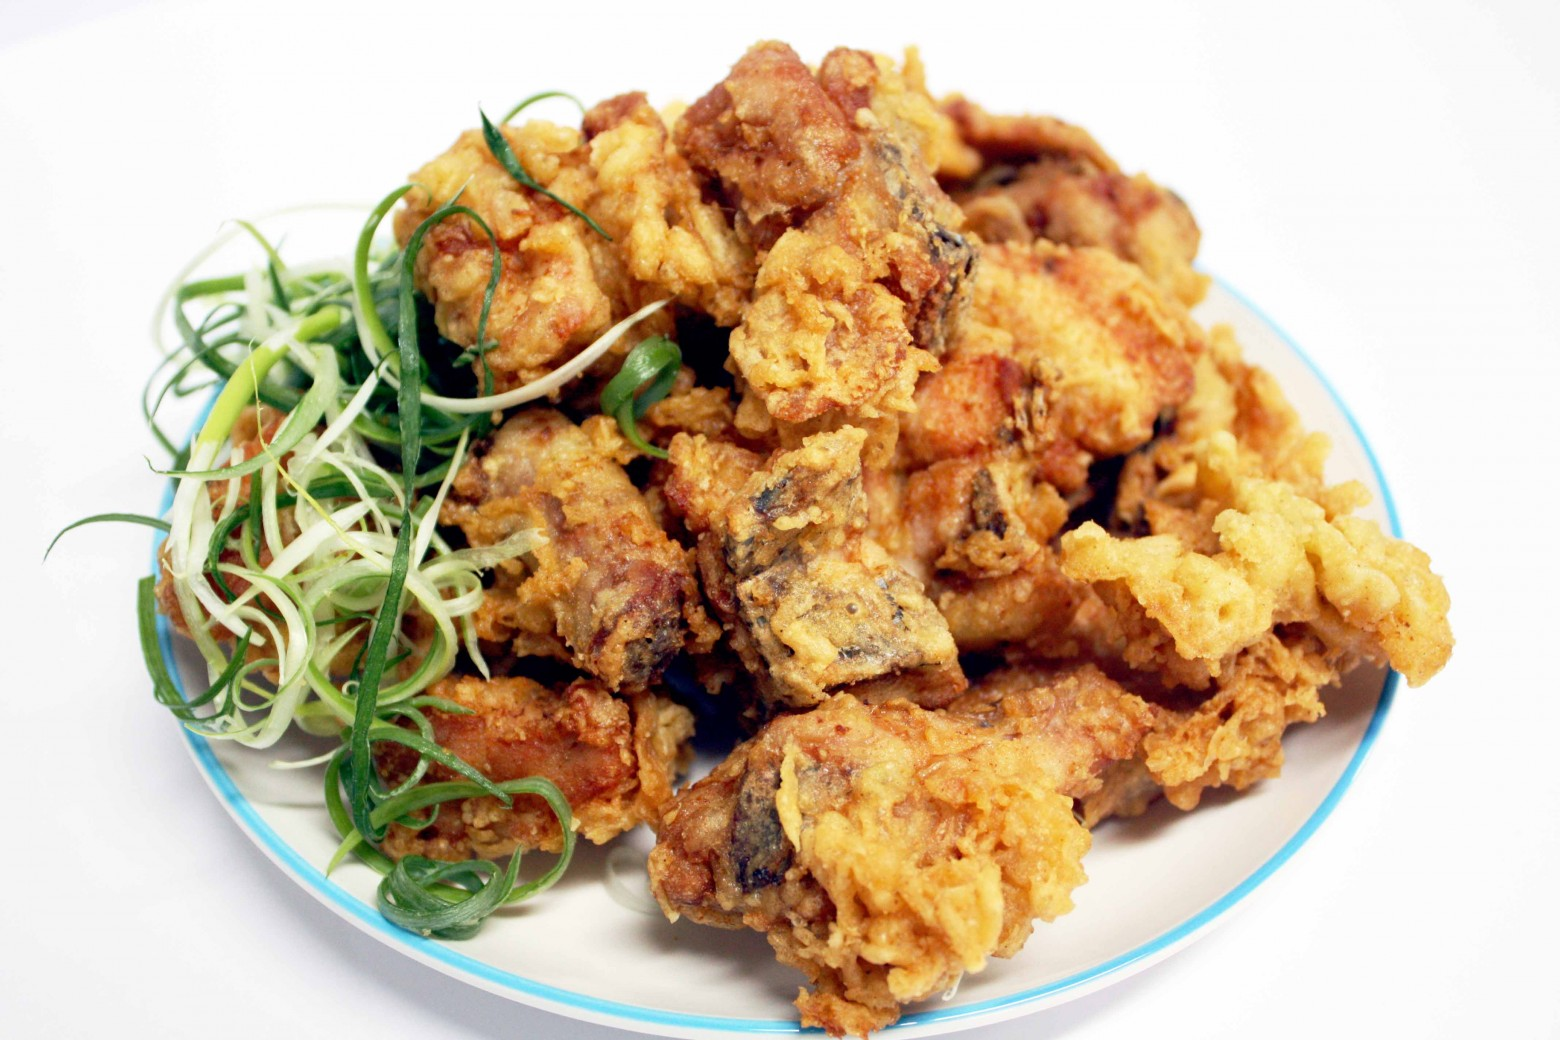
\includegraphics[width=0.8\textwidth]{chicken.jpg}
\end{center}

서울대학교 301동에는 아는 사람만 아는 ``눕치킨''이란 치킨집이 있다. 이 치킨집은 여느 치킨집처럼 치킨을 시킬 때 마다 쿠폰을 $C$장 주고, 쿠폰을 $F$장 모으면 치킨을 공짜로 시킬 수 있다.

눕치킨의 단골이 아닌 두영이에게는 쿠폰으로 시키는 치킨에는 쿠폰이 딸려나오지 않는다. 하지만 눕치킨의 단골 손님인 상언이에게는 치킨집 아저씨가 쿠폰으로 시키는 치킨에 쿠폰을 주신다. 상언이와 두영이는 둘 다 $M$원을 가지고 있고, 치킨의 가격은 $P$원이다. 이 때, 상언이는 두영이보다 치킨을 얼마나 더 시켜먹을 수 있을까?

\InputFile
첫 번째 줄에 테스트 케이스의 수 $T$ ($1 \le T \le 20,000$)가 주어지고, 이어서 $T$개의 테스트 케이스가 주어진다.

각 테스트 케이스마다 한 줄에 4개의 정수가 주어진다. 이는 순서대로
치킨의 가격 $P$ ($1 \le P \le 50,000$), 치킨에 쓸 돈 $M$ ($1 \le M \le 1,000,000$), 치킨을 공짜로 시키는데 필요한 쿠폰의 장수 $F$ ($2 \le F \le 1,000$), 치킨을 시키면 주는 쿠폰의 장수 $C$ ($1 \le C < F$) 를 의미한다.

\OutputFile
각 테스트 케이스마다, 첫 번째 줄에 상언이가 두영이보다 더 먹을 수 있는 치킨의 수를 출력한다.

\Example

\begin{example}
\exmp{2
10000 50000 5 1
10000 250000 5 1}{0
1}%
\end{example}

\end{problem}
